\subsection{Marcel Dzama Sergisi}
\indent\indent Marcel Dzama, şu anda New York'ta yaşayan 1974 Winnipeg doğumlu Kanadalı sanatçıdır. Çok yönlü bir sanatçı olan Dzama, ağırlık olarak resim, heykel, kağıt katlama, kısa film gibi alanlarda eserler üretmektedir.\newline
\indent Hayattaki deneyimlerinden beslenen Dzama'nın eserlerinde hayvan figürleri ön plana çıkıyor. Çocukluğunda dedesinin çiftliğinde ayı, geyik, yarasa, kokarca gibi hayvanları çok sık görmesinin etkisi olduğunu söylüyor. Bu hayvanlardan yarasalarla daha belirgin bir anısı var. İlkokulunda konteyner sınıflarda öğrenim gören Dzama, bir gün bu konteynerların fileyle sarılmış kısmını kesmeye heveslenir. Fileyi kesmesiyle beraber onlarca yarası kaçışır ve bu sahne Dzama üzerinde derin etki yaratır.\newline
\indent Bir diğer sık rastlanan motif ise ay. Çocukluğundan beri aya karşı bir ilgisi olduğunu belirten yazar, Meksika ve özellikle Fas'a yaptığı gezilerden sonra ay motifini daha çok kullandığını ekliyor. \textit{Blue Moon of Morroco} isminde bir sergisi ve \textit{To Live On The Moon(For Lorca)} isimli İspanyol şair Federico Garcia Lorca'ya ithaf ettiği kısa müzikal filmi bulunmaktadır.\newline
\indent Protest tarafını da resimlerinde sık sık ön plana çıkarmaktadır. Dünyadaki diktatörlüklere ve kötü yönetimlere karşı olan duruşunu sık sık vurguluyor. Eserlerinde Trump, Putin, Stalin gibi liderlere karikatürize edilmiş şekillerde rastlıyoruz. George Orwell'in 1984 romanına yaptığı göndermeler yine diktatörlük eleştirisi olarak göze çarpıyor.\newline
\indent Bir diğer eleştiri odağı ise patriarka. Eserlerinde kadınların daha ön plana çıkması gerektiğini, devrimin ve barışın kadınların ellerinden geleceğini ifade etmektedir. Özellikle \textit{The revolution will be female}(Devrim dişi olacak) ve \textit{Let the Women rule after the clown is through}(Palyaço gittikten sonra kadınlar yönetsin) isimli eserlerinde bu mesajlar daha açık görülmektedir.\newline
\begin{figure}[H]
    \centering
    \subfigure[The revolution will be female]{
        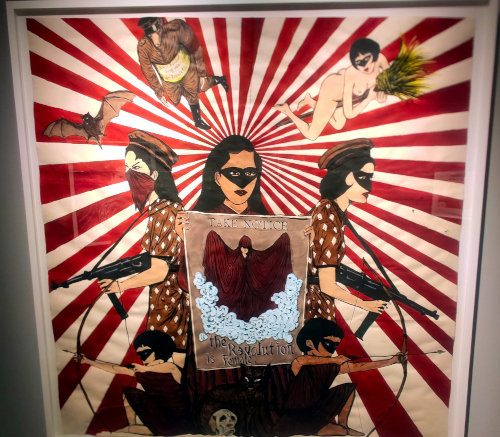
\includegraphics[width=0.45\linewidth]{assets/dzama_2.jpg}
    }
    \hfill
    \subfigure[Let the Women rule after the clown is through]{
        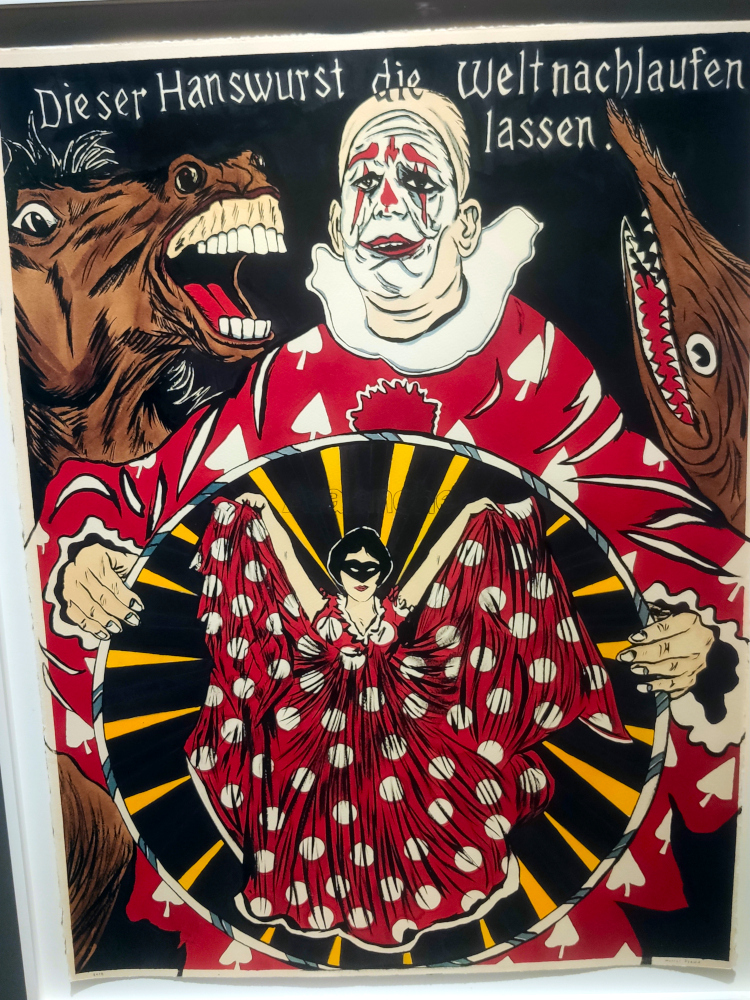
\includegraphics[width=0.30\linewidth]{assets/dzama_3.jpg}
    }
    \caption{Marcel Dzama'nın Protest Eserleri}
\end{figure}
\indent Joseph Beuys, Marcel Duchamp va dadaizm etkilerine eserlerinde sık sık rastlıyoruz. Kelime oyunlarını seven Dzama, \textit{Be little Beuys and Dada might buy you a Bauhaus} isimli eserindr \textit{boys} kelimesini \textit{Beuys} ve \textit{daddy} kelimesini \textit{dada} şeklinde yazarak Joseph Beuys ve dadaizme gönderme yapmaktadır. Öte yandan Marcel Duchamp'ın(kendisi iyi bir satranç oyuncusudur) satrançı eserlerinde kullanmaya başlamasından etkilenmiş; satranç ile savaş arasında ilgi kurarak heykellerinde ve kısa filmlerinde bu temayı işlemiştir.
\begin{figure}[H]
    \centering
    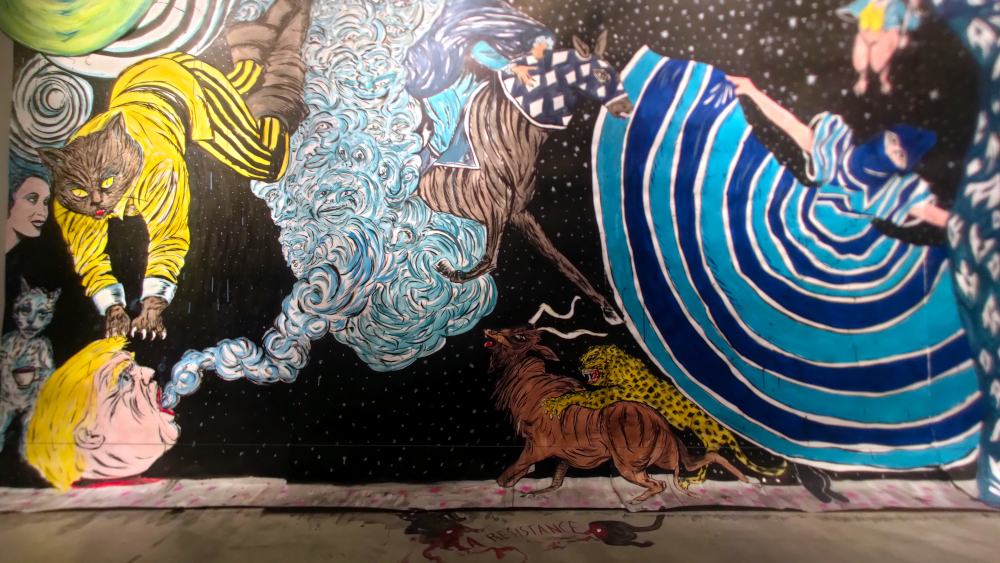
\includegraphics[width=0.9\linewidth]{assets/dzama_1.jpg}
    \caption{Be little Beuys and Dada might buy you a Bauhaus}
\end{figure}